\documentclass[a4paper,11pt]{article}
\usepackage[utf8]{inputenc}
%\usepackage{polski} 

\usepackage{apacite}
\usepackage{natbib}
\usepackage{hyperref} 
\usepackage[margin=1in]{geometry} 
\usepackage{amsmath,amsthm,amssymb}
\usepackage{graphicx}
\usepackage{subcaption}
\graphicspath{{images/}}


\newenvironment{theorem}[2][Theorem]{\begin{trivlist}
\item[\hskip \labelsep {\bfseries #1}\hskip \labelsep {\bfseries #2.}]}{\end{trivlist}}
\newenvironment{lemma}[2][Lemma]{\begin{trivlist}
\item[\hskip \labelsep {\bfseries #1}\hskip \labelsep {\bfseries #2.}]}{\end{trivlist}}
\newenvironment{exercise}[2][Exercise]{\begin{trivlist}
\item[\hskip \labelsep {\bfseries #1}\hskip \labelsep {\bfseries #2.}]}{\end{trivlist}}
\newenvironment{reflection}[2][Reflection]{\begin{trivlist}
\item[\hskip \labelsep {\bfseries #1}\hskip \labelsep {\bfseries #2.}]}{\end{trivlist}}
\newenvironment{proposition}[2][Proposition]{\begin{trivlist}
\item[\hskip \labelsep {\bfseries #1}\hskip \labelsep {\bfseries #2.}]}{\end{trivlist}}
\newenvironment{corollary}[2][Corollary]{\begin{trivlist}
\item[\hskip \labelsep {\bfseries #1}\hskip \labelsep {\bfseries #2.}]}{\end{trivlist}}





\author{Student: Karan Daei-Mojdehi\\*Instructor: Dr. Guo-Jin Qi\\* University of Central Florida}
\title{Knowledge Representation Machine Problem 2:\\* Logistic Regression: Learning and Inference }
\date{\today}

\begin{document}
\maketitle


\section*{Introduction}
In this Machine Problem, we are requested to implement a Logistic Regression Learning Algorithm on a previously chosen data set from UCI machine learning website. Batch and stochastic gradient descent training are explored and evaluated as well as effect of adding a L2 regularization term to likelihood function. At the end, performance of Logistic Regression on our data set is compared to that of a decision tree which was implemented in previous machine problem.

\section*{Step 1: The Data Set}
As suggested, I used the same data set for previous assignment which included information about adults salary with goal of predicting whether their salary is +\$50k or not. This data set includes both categorical and numerical attributes and is made up of 48000 instances. As suggested, categorical data are coded into binary vector to make implementation of Logistic Regression possible. This problem will be a binary classification task. Output label of +1 corresponds to a +\$50k salary, while label of -1 is used for salaries below \$50k.The data set can be found online  
\href{<https://archive.ics.uci.edu/ml/datasets/Adult.>}{<Here>}. 


\section*{Step 2: Implementation of Batch LR model}
LR model is made up of a number of weights ( equal to total number of attributes in our data set after binary vectorization in addition to a bias ) and a likelihood function which foretells label of an input data by computing the following probability:
\begin{equation}
 P(Y=1 | X ) = \frac{1}{1 + exp(\sum_{i=1}^{N}-W^TX_i)} 
\end{equation}
in which $X_i$ is a border of attributes of entry i and W is a vector of our model weights. For training of the LR model, likelihood is defined as probability of our LR model (weights) successfully predicting probability of labels all samples in our data set.Likelihood can be calculated using following equation:
\begin{equation}
 Likelihood( Weights )\newline
 =\prod_{X_i:Y_i=1}\frac{1}{1 + exp(\sum_{i=1}^{N}-W^TX_i)}  . \prod_{Xj:Y_j=-1}1-\frac{1}{1 + exp(\sum_{j=1}^{N}-W^TX_j)} \\
\end{equation}
\begin{equation}\label{something}
= \prod_{i=1}^{N} \frac{1}{1 + exp(\sum_{i=1}^{N}-Y_iW^TX_i)} 
\end{equation}

where $Y_i$ is the ground truth label assigned to $X_i$ which is +1 for True entries and -1 for False entries. Log likelihood will be natural logarithm of above introduced function which will be equal to:
\begin{equation}
LogLikelihood ( Weights )  = - \sum_{i=1}^{N}ln(1+exp(-Y_iW^TX_i))
\end{equation}
Now we use the gradient descent method to optimize likelihood of our model with respect to our model parameters ( Weights ). By taking derivative with respect to W and some simplifications, we will have:
\begin{equation}
\nabla _W LL (W) = \sum_{i=1}^{N}\frac{Y_iX_i}{1+exp(Y_iW^TX_i)} 
\end{equation}
In order to train the LR model, we update weights of the model iteratively in the direction of gradient ascent ( 'ascent' since we are maximizing likelihood ) with a factor = $\eta$, also known as learning rate. In Batch mode training we look at all the training data in each iteration to extract update rule for weights, i.e. our update rule will be:
\begin{equation}
W\textrm{nextIteration} = W\textrm{currentIteration} + \eta \nabla _W LL(W)
\end{equation}
This iterative update continues until one of the below stop criteria are detected:\\
a) number of iterations exceed a constant (MAX\underline{\hspace{.2cm}}ITERS) \\
b) the difference between two consequent iterations' weights drops below a certain threshold (TH\underline{\hspace{.2cm}}MIN\underline{\hspace{.2cm}}W\underline{\hspace{.2cm}}UPDATE) which is equivalent to detecting a certain amount of drop in gradient of log likelihood ( we are using $\nabla _W LL (W)$ to update weights).\newline
Also log likelihood in each iteration is compared to it's previous one and in case it is lower that previous step, learning rate temporary shrinks to one fifth of it's original size in that iteration. 
\begin{figure}[t]

\begin{subfigure}{.5\textwidth}

  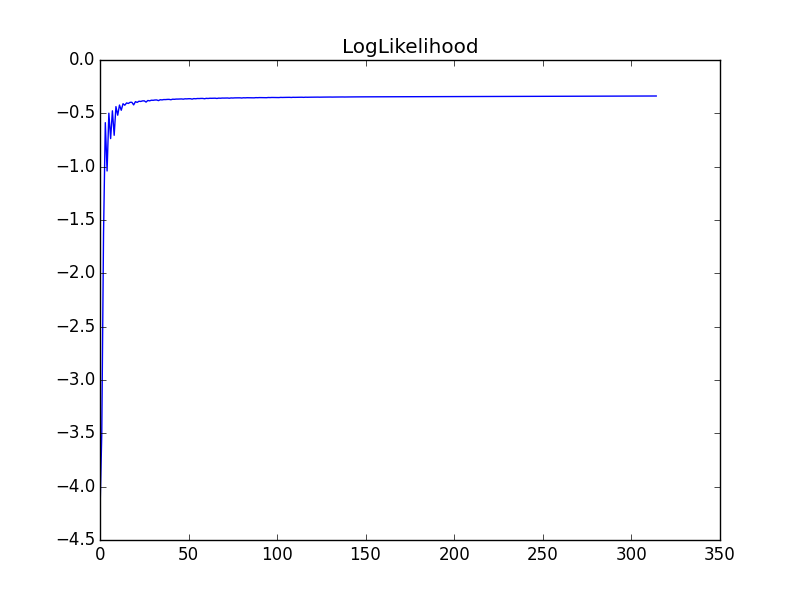
\includegraphics[width=1\linewidth]{images/LLBatch_iter315_eta5_numIns32560.png}
	\centering
  \caption{log likelihood }
  \label{fig:batch_loglikelihood}
\end{subfigure}
\begin{subfigure}{.5\textwidth}

  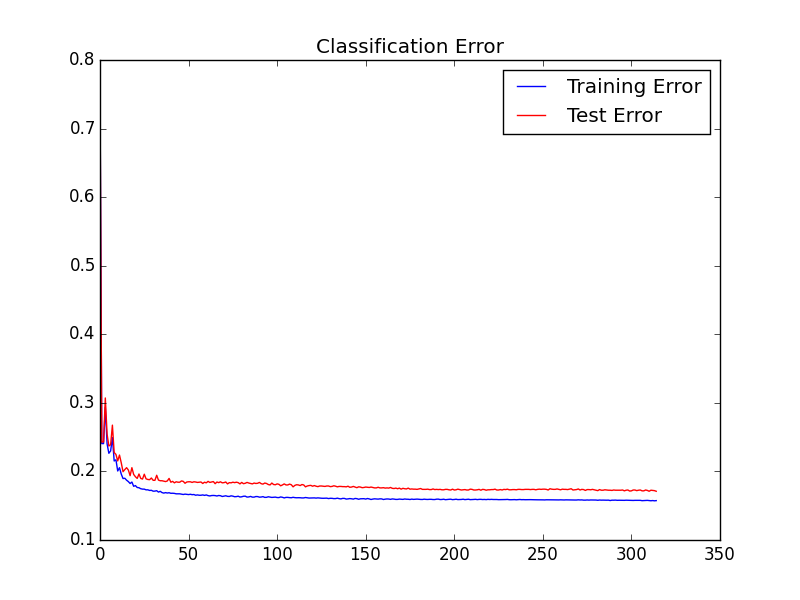
\includegraphics[width=1\linewidth]{images/testError_Batch_iter315_eta5_numIns32560.png}
	\centering
  \caption{test and train error }
  \label{fig:batch_errors}
\end{subfigure}

  \caption{Batch Training Results}
\end{figure}

Figure \ref{fig:batch_loglikelihood} shows log likelihood over iterations in a batch training run of our LR model. We observe that over iterations, our LR model become more probable ('likely') to estimate labels of our training data which means the model is learning. By a closer look at this figure, we can tell that learning rate is tuned correctly since log likelihood is monotonically increasing over iteration and converges in relatively short number of iterations. An inappropriate learning rate would had resulted in either fluctuation ( a large learning rate ) or slow convergence ( small learning rate ) in log likelihood. A smaller learning rate will smooth out the large fluctuations in early iterations before convergence, but will increase the number of iterations until stagnation.
Figure(\ref{fig:batch_errors} ) shows how test and train error decrease over iterations and stagnate when training converges. In this run all data samples where used for our task and was divided into 10 folds. Nine out of ten folds were used for training and test results are reported for the fold that was left out of training. After convergence accuracy on train and test data data 84\% and 83.9\% , True Positive Rate (TPR) was 55.35\% and 55.31\% , and True Negative rate (TNR) was 93.15\% and 92.79\% for train and test data. These measures shows a bias toward Negative labels in our data set. By comparing performance on test and train data and errors over iterations over those data in Figure(\ref{fig:batch_errors}), we can assert that our LR model is not being over-fit on our train data. Main reasons behind this is our huge train data size, which we reduce in step 4 in order to observe over-fitting and how it's affected by regularization.

\section*{Step 3: Implementation of Stochastic Gradient Ascent (SGA) LR model}
In order to change our learning algorithm from Batch learning to SGA, all we need to do is randomly choose a relatively small subset of our training data and compute likelihood and its gradient over this small subset in each iteration. Huge advantage of this method lies in reduction in complexity of computations in each step, since we don't have to compute likelihood in each iteration ( although in this assignment, for reporting purposes, still log likelihood is calculated and stored in each iteration ). Tuning of learning rate (SGA\underline{\hspace{.2cm}}ETA) and size of randomly chosen subset (SGA\underline{\hspace{.2cm}}SAMPLE\underline{\hspace{.2cm}}SIZE) is essential to convergence of SGA method. A smaller subset would require a smaller learning rate since it's information is less reliable while a larger one includes more reliable information and therefore can exploit a larger learning rate. Rest of the steps are the same as batch learning. \\ 
\begin{figure}[t]
\begin{subfigure}{.5\textwidth}
  \includegraphics[width=1\linewidth]{images/LLSGA_samplesize40_eta0_3_numIns32560.png}
	\centering
  \caption{log likelihood }
  \label{fig:SGA40_loglikelihood}
\end{subfigure}
\begin{subfigure}{.5\textwidth}
  \includegraphics[width=1\linewidth]{images/testError_SGA_samplesize40_eta0_3_numIns32560.png}
	\centering
  \caption{test and train error }
  \label{fig:SGA40_errors}
\end{subfigure}
  \caption{SGA Training Results, SGA\underline{\hspace{.2cm}}SAMPLE\underline{\hspace{.2cm}}SIZE = 40 , SGA\underline{\hspace{.2cm}}ETA = 0.3}
  \label{fig:SGA40}
\end{figure}

Figure \ref{fig:SGA40} shows results from SGA training and its evaluation on test data set with subset size of 40 and learning rate of 0.3. Log likelihood in \ref{fig:SGA40_loglikelihood} is monotonically increasing towards 0 which shows SGA LR is learning with an appropriate learning rate. In this run, Accuracy, TPR, and NPR were 83.38\%, 59.74\%, and 90.87\% on train set and 83.78\%, 60.15\%, and 91.3\% on test set respectively. Again large size of our training data and relatively small test data set has swept away over-fitting problem. In another run with the same learning rate but subset of sizes 10 and 3 (Figures \ref{fig:SGA10} and \ref{fig:SGA3} respectively), we can observe that weights move in more diverse directions in each iteration and therefore result in a fluctuation in likelihood and classification error on both test and train data set. Although Classification evaluation results exceed the ones from runs with larger subset size in some runs, they are not reliable and have a $\pm$ 10\% fluctuation. A smaller learning rate in these runs would had reduced these fluctuations.

\begin{figure}[t]

\begin{subfigure}{.5\textwidth}

  \includegraphics[width=1\linewidth]{images/LLSGA_samplesize10_eta0_3_numIns32560.png}
	\centering
  \caption{log likelihood }
  \label{fig:SGA10_loglikelihood}
\end{subfigure}
\begin{subfigure}{.5\textwidth}

  \includegraphics[width=1\linewidth]{images/testError_SGA_samplesize10_eta0_3_numIns32560.png}
	\centering
  \caption{test and train error }
  \label{fig:SGA10_errors}
\end{subfigure}

  \caption{SGA Training Results, SGA\underline{\hspace{.2cm}}SAMPLE\underline{\hspace{.2cm}}SIZE = 10 , SGA\underline{\hspace{.2cm}}ETA = 0.3}
  \label{fig:SGA10}
\end{figure}

\begin{figure}[t]

\begin{subfigure}{.5\textwidth}

  \includegraphics[width=1\linewidth]{images/LLSGA_samplesize3_eta0_3_numIns32560.png}
	\centering
  \caption{log likelihood }
  \label{fig:SGA3_loglikelihood}
\end{subfigure}
\begin{subfigure}{.5\textwidth}

  \includegraphics[width=1\linewidth]{images/testError_SGA_samplesize3_eta0_3_numIns32560.png}
	\centering
  \caption{test and train error }
  \label{fig:SGA3_errors}
\end{subfigure}

  \caption{SGA Training Results, SGA\underline{\hspace{.2cm}}SAMPLE\underline{\hspace{.2cm}}SIZE = 3 , SGA\underline{\hspace{.2cm}}ETA = 0.3}
  \label{fig:SGA3}
\end{figure}


\section*{Step 4: Adding Regularization Term}
Adding a regularization term will prevent a model from fully fitting a train data set and is mainly used to avoid over-fitting. Regularization is done with goal of reaching a better out of sample performance by avoiding fully 'memorizing' training date, therefore we expect to witness a decrease in in-sample performance.Adding an $L_2$ regularizer to the log likelihood function will result in the new cost function:
 \begin{equation}
LogLikelihood ( Weights )  = - \sum_{i=1}^{N}ln(1+exp(-Y_iW^TX_i)) -\frac{1}{2\sigma^2} ||W||^2 
\end{equation}
By taking gradient of the new log likelihood function, we arrive at the new update rule for regularized learning:
\begin{equation}
\nabla _W LL (W) = \sum_{i=1}^{N}\frac{Y_iX_i}{1+exp(Y_iW^TX_i)} - \frac{1}{\sigma^2} W
\end{equation}
\begin{equation}
W\textrm{nextIteration} = W\textrm{currentIteration} + \eta \nabla _W LL(W)
\end{equation}
\subsection*{Batch Regularization}
Before adding a regularizer, note that as observed in previous steps, the portion of data that we are using for training of our model is huge and we are not observing any over-fitting in the first place. Therefore, I first decreased training data set size portion and also discarded large portion of available data ( reduced total available instances to 800) and used half of those data for training and the other half for test in order to make the conditions more likely for over-fitting the model. I also increased maximum number of iterations as well as threshold in minimum required update in weights for each iteration. Figure \ref{fig:Batch_overfit} shows results of my success in over-fitting the data. By looking at Figure \ref{fig:Batch_overfit error} we can see that the model starts over-fitting at iterations around 70 since train error is still decreasing while test error starts rising.  
\begin{figure}[t]

\begin{subfigure}{.5\textwidth}

  \includegraphics[width=1\linewidth]{images/LLBatch_iter700_eta5_0_numIns800.png}
	\centering
  \caption{log likelihood }
  \label{fig:LLBatch_overfit}
\end{subfigure}
\begin{subfigure}{.5\textwidth}

  \includegraphics[width=1\linewidth]{images/testError_Batch_iter700_eta5_0_numIns800.png}
	\centering
  \caption{test and train error }
  \label{fig:Batch_overfit error}
\end{subfigure}

  \caption{Batch over-fit Training Results, folds = 2 , ETA = 5, no regularizer}
  \label{fig:Batch_overfit}
\end{figure}
 Now is the time to observe effect of adding a regularizer. while keeping all other parameters fixed, vary sigma from 1 to 100 , and perform 10 runs of training for each sigma ( on random samples from the huge pool of data set), Figure \ref{fig:ValidBatch_reg} shows the average of error on validation set for different values of sigma. With this values and corresponding average error in mind, we set sigma value to 50 and 70 and evaluate effect of regularizer term on over-fitting.  

\begin{figure}[b]
  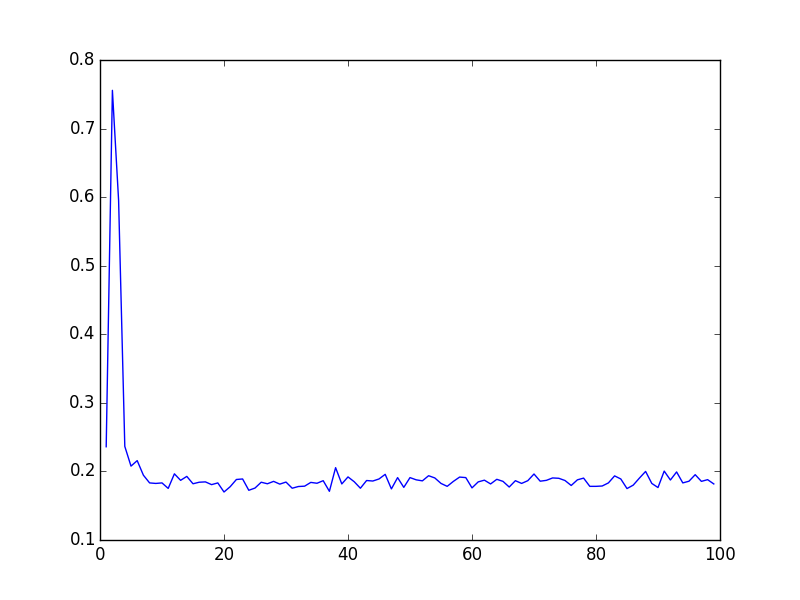
\includegraphics[width=.5\linewidth]{images/BatchValid.png}
	\centering
  \caption{Average Validation Error over Sigma (Batch Regularization)}
  \label{fig:ValidBatch_reg}
\end{figure}
\newpage
Figures \ref{fig:Batch_reg_sig50_er} and \ref{fig:Batch_reg_sig70_er} show classification error over iterations. We can observe that regularization is taking effect: although error on training set has slightly increased, ( compare it to Figure \ref{fig:Batch_overfit error} ) , error on test data set is lower and it does not increase beyond any iteration (so far). Clearly we can assert that regularization doesn't permit our model to over-fit. 
\begin{figure}[t]
\begin{subfigure}{.5\textwidth}
  \includegraphics[width=1\linewidth]{images/testError_Batch_iter700_eta5_0_numIns800_sig50.png}
	\centering
  \caption{Error with Regularization, SIGMA = 50 }
  \label{fig:Batch_reg_sig50_er}
\end{subfigure}
\begin{subfigure}{.5\textwidth}
  \includegraphics[width=1\linewidth]{images/testError_Batch_iter700_eta5_0_numIns800_sig70.png}
	\centering
  \caption{Error with Regularization, SIGMA = 70 }
  \label{fig:Batch_reg_sig70_er}
\end{subfigure}
  \caption{Regularized Batch Training Error Results, ETA = 5}
  \label{fig:BatchReg}
\end{figure}
Log likelihood in these runs are plotted in Figure \ref{fig:LLBatchReg} and show that the regularizer with sigma =70 results in less fluctuation in loglikelihood and is more stable after convergence. 
\begin{figure}[t]
\begin{subfigure}{.5\textwidth}
  \includegraphics[width=1\linewidth]{images/LLBatch_iter700_eta5_0_numIns800_sig50.png}
	\centering
  \caption{ SIGMA = 50 }
  \label{fig:Batch_reg_sig50_LL}
\end{subfigure}
\begin{subfigure}{.5\textwidth}
  \includegraphics[width=1\linewidth]{images/LLBatch_iter700_eta5_0_numIns800_sig70.png}
	\centering
  \caption{ SIGMA = 70 }
  \label{fig:Batch_reg_sig70_LL}
\end{subfigure}
  \caption{Regularized Batch Training LogLikelihood Results, ETA = 5}
  \label{fig:LLBatchReg}
\end{figure}

\subsection*{Stochastic Gradient Ascent Regularization}
Same as Batch regularized section, first we try to arrive at over-fit results without a regularizer and then add a regularizer term to examine effect of regularization. Every step for regularization of SGA is same as Batch method, except that for reporting purposes, we calculate error and likelihood not only for randomly selected subset of training data, but also for whole training data and test data. I reduced total available number of instances to 500 and maximum number of iterations to 5000 in order to make the conditions suitable for over-fitting. Figure \ref{fig:SGA_overfit} shows log likelihood and error in this run. It is clear that our SGA method is over-fitting the model since test error starts rising after iteration 800.


\begin{figure}[t]
\begin{subfigure}{.5\textwidth}
  \includegraphics[width=1\linewidth]{images/LLSGA_iters5010_samplesize40_eta0_3_numIns500_sig666.png}
	\centering
  \caption{log likelihood }
  \label{fig:LLSGA_overfit}
\end{subfigure}
\begin{subfigure}{.5\textwidth}
  \includegraphics[width=1\linewidth]{images/testError_SGA_iters5010_samplesize40_eta0_4_numIns500_sig666.png}
	\centering
  \caption{test and train error (note over-fitting) }
  \label{fig:SGA40_overfit_er}
\end{subfigure}
  \caption{SGA Training Results, SGA\underline{\hspace{.2cm}}SAMPLE\underline{\hspace{.2cm}}SIZE = 40 , SGA\underline{\hspace{.2cm}}ETA = 0.3}
  \label{fig:SGA_overfit}
\end{figure}
\newpage
Now that we know our model over-fits in these conditions, we fix our training parameters, and  follow the same procedure as Batch regularization. Figure \ref{fig:SGA_reg_valid} shows results of adding a regularizer to our update rule for sigmas in range of 1 to 100.

\begin{figure}[b]
  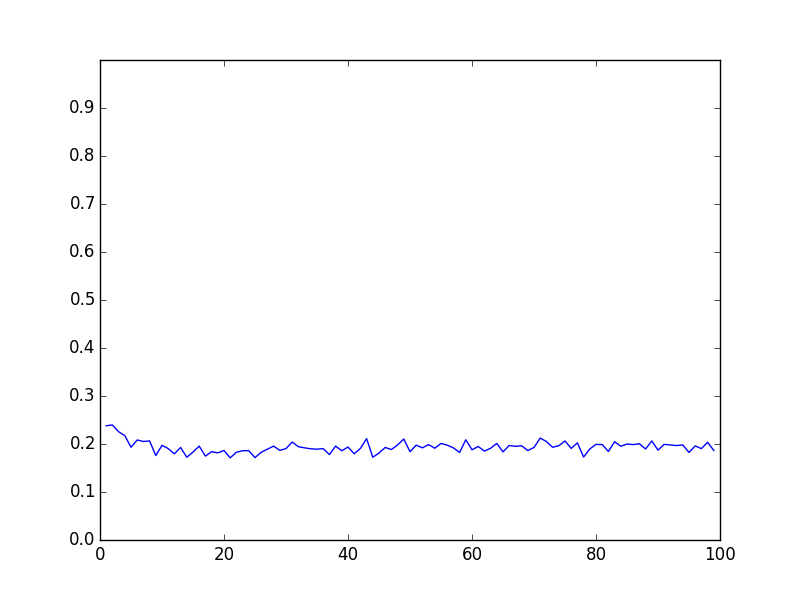
\includegraphics[width=.5\textwidth]{images/SGAVALID.png}
	\centering
  \caption{Average Validation Error over Sigma (SGA Regularization) }
  \label{fig:SGA_reg_valid}
\end{figure}

According to Figure \ref{fig:SGA_reg_valid} , we choose sigma value of 15 (SIGMA = 15)and plot the results in Figure \ref{fig:SGA_sig15}. As we were hopping, we can perceive that again adding a regularizer has decreased our performance on training error (compare with Figure\ref{fig:SGA40_overfit_er}, but results in a better classification on test data set. We can also note that signs of over-fitting have vanished in these runs thanks to regularizer term. Log likelihood and classification error are plotted for other values of sigma in figures \ref{fig:SGA_sig45} to \ref{fig:SGA_sig90} . By observing log likelihood, we can note that smaller values of sigma will result in a poor log likelihood ( which is a measure of how much our model fits the training data) and increasing sigma will enhance log likelihood over training data and allows our model to better fit training data, while increasing chances of over-fitting.
% sigma = 15:
\begin{figure}[t]
\begin{subfigure}{.5\textwidth}
  \includegraphics[width=1\linewidth]{images/LLSGA_iters5010_samplesize40_eta0_3_numIns500_sig15.png}
	\centering
  \caption{log likelihood }
  \label{fig:LLSGA_sig15}
\end{subfigure}
\begin{subfigure}{.5\textwidth}
  \includegraphics[width=1\linewidth]{images/testError_SGA_iters5010_samplesize40_eta0_3_numIns500_sig15.png}
	\centering
  \caption{test and train error  }
  \label{fig:SGA40_sig15_er}
\end{subfigure}
  \caption{SGA Regularized Training Results, SGA\underline{\hspace{.2cm}}ETA = 0.3, SIGMA = 15}
  \label{fig:SGA_sig15}
\end{figure}
% sigma = 45
\begin{figure}[t]
\begin{subfigure}{.5\textwidth}
  \includegraphics[width=1\linewidth]{images/LLSGA_iters5010_samplesize40_eta0_3_numIns500_sig45.png}
	\centering
  \caption{log likelihood }
  \label{fig:LLSGA_sig45}
\end{subfigure}
\begin{subfigure}{.5\textwidth}
  \includegraphics[width=1\linewidth]{images/testError_SGA_iters5010_samplesize40_eta0_3_numIns500_sig45.png}
	\centering
  \caption{test and train error }
  \label{fig:SGA40_sig45_er}
\end{subfigure}
  \caption{SGA Regularization Training Results, SGA\underline{\hspace{.2cm}}ETA = 0.3 , SIGMA = 45}
  \label{fig:SGA_sig45}
\end{figure}
% sigma =75
\begin{figure}[t]
\begin{subfigure}{.5\textwidth}
  \includegraphics[width=1\linewidth]{images/LLSGA_iters5010_samplesize40_eta0_3_numIns500_sig75.png}
	\centering
  \caption{log likelihood }
  \label{fig:LLSGA_sig75}
\end{subfigure}
\begin{subfigure}{.5\textwidth}
  \includegraphics[width=1\linewidth]{images/testError_SGA_iters5010_samplesize40_eta0_3_numIns500_sig75.png}
	\centering
  \caption{test and train error }
  \label{fig:SGA40_sig75_er}
\end{subfigure}
  \caption{SGA Training Results, SGA\underline{\hspace{.2cm}}ETA = 0.3, SIGMA = 75}
  \label{fig:SGA_sig75}
\end{figure}
%sigma = 90
\begin{figure}[t]
\begin{subfigure}{.5\textwidth}
  \includegraphics[width=1\linewidth]{images/LLSGA_iters5010_samplesize40_eta0_3_numIns500_sig90.png}
	\centering
  \caption{log likelihood }
  \label{fig:LLSGA_sig90}
\end{subfigure}
\begin{subfigure}{.5\textwidth}
  \includegraphics[width=1\linewidth]{images/testError_SGA_iters5010_samplesize40_eta0_3_numIns500_sig90.png}
	\centering
  \caption{test and train error  }
  \label{fig:SGA40_sig90_er}
\end{subfigure}
  \caption{SGA Regularized Training Results,SGA\underline{\hspace{.2cm}}ETA = 0.3, SIMA = 90}
  \label{fig:SGA_sig90}
\end{figure}




\newpage
\section*{Step 5: Report and Comparison with Decision Tree}
By comparing evaluation results from original runs ( no the runs in which we had  intentionally over-fit the models) we observe that logistic regression has a slightly lower overall accuracy, while it has a better TNR (True Negative Rate). Having in mind that our data set is more biased toward Negative samples, we can tell that performance of logistic regression is more better on the selected data set. This can be mainly due to inability of decision to monitor all of attributes at the same time and make a decision on a combination of them, i.e. correlation between attributes of our data set is captured better by the LR model. 


















\end{document}